\setcounter{page}{1}
\pagenumbering{arabic}
\chapter{Inleiding}
\label{ch:Inleiding}
Menselijke actieherkenning is het proces dat op een automatische manier (I) detecteert dat een persoon een bepaalde actie uitvoert en (II) herkennen welke actie dit is. Voorbeelden van zulke acties zijn lopen, stappen, zwaaien, springen, bukken, enz. Actieherkenning kent tal van toepassingen, voornamelijk bij de interactie tussen mens en computer, zoals fysiotherapie \cite{Deboeverie2016}, lichaamsanalyse \cite{Devi2015} en \todo{nog wat voorbeelden zoeken}

Actieherkenning wordt voornamelijk gerealiseerd met kleuren- en dieptebeelden.







\section{Probleemstelling}
In het onderzoeksgebied actieherkenning is er al uitbundig onderzoek gedaan. Zo is men in staat om voor zowel kleurenbeelden als dieptebeelden 

In de literatuur wordt er vaak een speciale pose, de startpose, verwacht \cite{Zhu2013}, \cite{Deboeverie2016}. Dit is de pose die een persoon moet aannemen vooraleer actieherkenning uitgevoerd zal worden.

Actieherkenning en actiedetectie blijft moeilijk te realiseren in een real-time scenario, waarbij snelle beslissingen gemaakt moeten worden. Het doel van deze masterproef is om eerst te onderzoeken welke methoden er al bestaan op vlak van actieherkenning en hoe deze efficiënter kunnen gemaakt worden. De algemene aanpak wordt beschreven in hoofdstuk \ref{ch:methodologie}.



\section{De Kinect}
De Kinect (figuur \ref{fig:KinectSensorVersies}) is origineel ontworpen als manier om de gebruiker zelf als spelcontroller te beschouwen. Voor deze masterproef wordt de tweede versie van de Kinect gebruikt (figuur \ref{fig:KinectSensorOne}) en wordt kort besproken.

De Kinect bevat meerdere sensoren waaronder een kleurencamera, dieptecamera en infraroodcamera. Op basis van de dieptebeelden is de Kinect in staat om een skelet te genereren voor maximaal zes personen, elk met 25 joints die belangrijke kenmerken van het menselijk lichaam voorstellen, meestal op de plaats van gewrichten.


\begin{figure}
	\begin{subfigure}[t]{0.48\textwidth}
		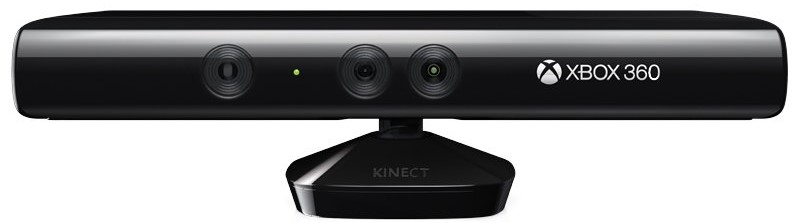
\includegraphics[width=\linewidth]{KinectSensor360}
		\caption{De originele Kinect sensor, ontwikkeld int 2010 voor de Xbox 360.}
	\end{subfigure}
	\begin{subfigure}[t]{0.48\textwidth}
		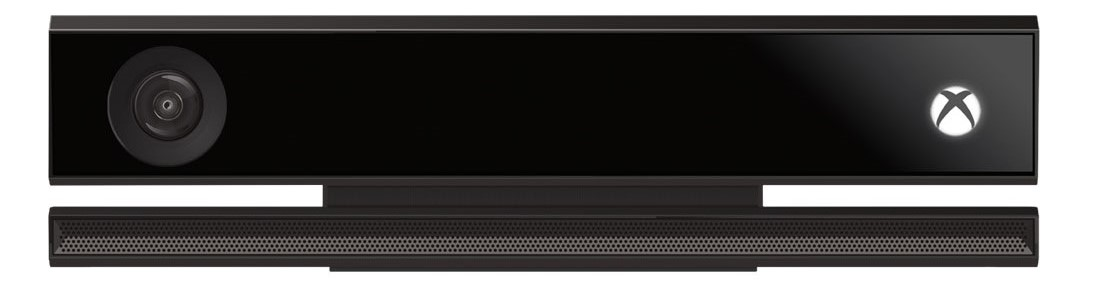
\includegraphics[width=\linewidth]{KinectSensorOne}
		\caption{De tweede iteratie van de Kinect sensor, specifiek gemaakt voor Xbox One en uitgebracht in 2013.}
		\label{fig:KinectSensorOne}
	\end{subfigure}
	\caption{Twee versies van de Kinect sensor.}
	\label{fig:KinectSensorVersies}
\end{figure}




\section{Structuur}
In hoofdstuk \ref{ch:methodologie} wordt de algemene methodologie beschreven die gebruikt wordt om deze masterproef te realiseren, waarom deze gebruikt wordt en wat het beoogde eindresultaat is. Verder wordt er in hoofdstuk \ref{ch:literatuur} een overzicht gegeven van bestaande methoden en welke features en classifiers zij gebruiken.
